\section{Circuito implementado}
Nesta secção será descrito o processo de implementação física do projeto, ou seja, a montagem do sensor com a placa de desenvolvimento \textit{Arduino Uno}.

Para a montagem do sensor na placa de desenvolvimento, foi necessário saber qual era a característica do sinal de saída do sensor, para ligar o sensor num porto digital ou analógico. O sensor NTC possui na saída um sinal analógico correspondente a uma variação de tensão. Logo o sensor será ligado a uma entrada analógica com a configuração da Figura \ref{fig:NTCmontagem}. O esquema de ligações do circuito com a placa de desenvolvimento e sensor encontra-se na Figura \ref{fig:CircuitoTotal}.
\begin{figure}[!htb]
    \centering
    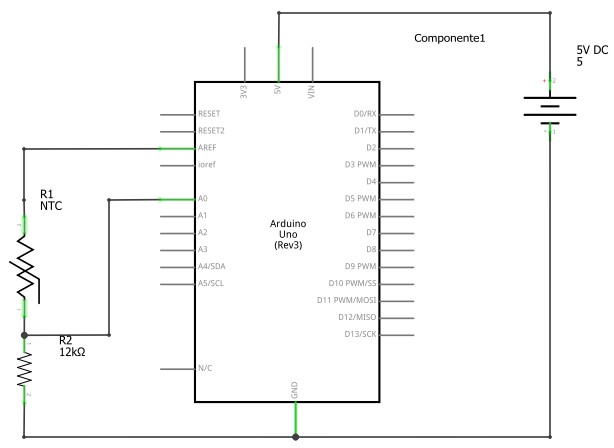
\includegraphics[width=0.7\textwidth]{img/Esquema_de_ligacoes.PNG}
    \caption{Esquema de ligações do sensor na placa de desenvolvimento.}
    \label{fig:CircuitoTotal}
\end{figure}

No código foi definido a resolução da entrada analógica, tendo esta um baud rate de 9600.

A alimentação do circuito é feito internamente, ou seja, é ligado um carregador que fornece 12V DC à placa de desenvolvimento e por meio de um regulador de tensão a tensão é convertida de 12V DC em 5V DC. Na Figura \ref{fig:CircuitoTotal} a alimentação da placa de desenvolvimento está representada por uma fonte de tensão de 5V DC.

No circuito foi colocado uma resistência no divisor de tensão com o sensor NTC de \(12k\Omega\) por lapso, isto porque a resistência devia de ter um valor de \(10k\Omega\), visto o valor referido na folha de especificações do sensor para a resistência uma temperatura de referência de \(25ºC\) ser de \(10k\Omega\). Para ultrapassar este problema, foi colocado no código que o valor da resistência era de \(12k\Omega\), mais concretamente \(12129.0\Omega\), porque o valor da resistência foi medido com um multímetro. Após se ter aplicado este método, foi possível obter valores de temperatura mais precisos.